
% This LaTeX was auto-generated from an M-file by MATLAB.
% To make changes, update the M-file and republish this document.

\documentclass{article}
\usepackage{graphicx}
\usepackage{color}

\sloppy
\definecolor{lightgray}{gray}{0.5}
\setlength{\parindent}{0pt}

\begin{document}

    
    
\section*{Loading and pre-processing of ALIS data}


\subsection*{Contents}

\begin{itemize}
\setlength{\itemsep}{-1ex}
   \item Typical steps in reading ALIS images
   \item Raw image reading
   \item For fits files with LE byte order: fits1
   \item ...and for files in BE byte order: fits2
   \item Standard ALIS data reading
   \item ALIS image pecularities
   \item Overscan strips
   \item Bad-border
   \item "Bad-pixels"
   \item Pre-processing
   \item Quadrant balancing
   \item Adjusting the image borders
   \item Correcting bad pixels
   \item All in one go.
\end{itemize}


\subsection*{Typical steps in reading ALIS images}

\begin{par}
Lets look at a typical image. First move to a data directory.
\end{par} \vspace{1em}
\begin{verbatim}
cd /home/bjorng/ursaminor/Data/alis_fast/970216
filename = '62G00017.RAF';
\end{verbatim}


\subsection*{Raw image reading}

\begin{par}
There are 2 functions for raw reading of images in fits format. (except the later 'fitsread' provided by mathworks, which is slower...)
\end{par} \vspace{1em}


\subsection*{For fits files with LE byte order: fits1}

\begin{verbatim}
[h,d] = fits1(filename);
imagesc(d)
title('image opened assuming wrong byte order','fontsize',16)
\end{verbatim}

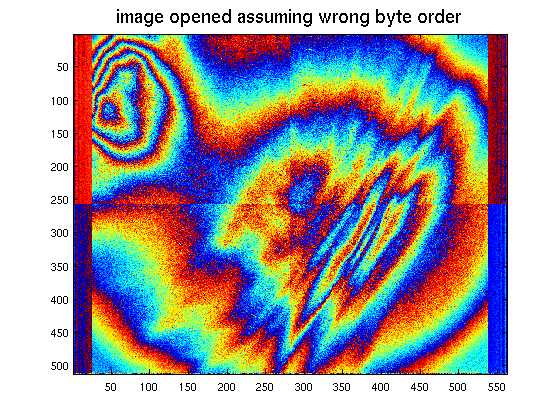
\includegraphics [width=4in]{ADA_1_loadnpreproc_p_01.png}


\subsection*{...and for files in BE byte order: fits2}

\begin{verbatim}
[h,d] = fits2(filename);
imagesc(d)
title('...and with the correct guess','fontsize',16)
caxis([-25066 -23866])
\end{verbatim}

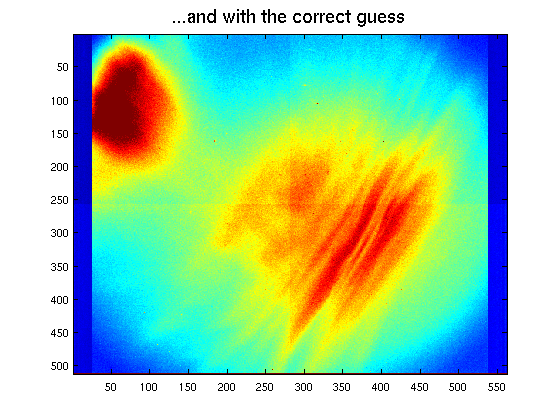
\includegraphics [width=4in]{ADA_1_loadnpreproc_p_02.png}


\subsection*{Standard ALIS data reading}

\begin{par}
There is a function that automatically chooses the right version: \texttt{inimg}. \texttt{inimg} also extracts the image header and even produces a structure with the relevant information more easily accesible
\end{par} \vspace{1em}
\begin{verbatim}
[d,h,o] = inimg(filename);
o = o
\end{verbatim}

\color{lightgray} \begin{verbatim}o = 
        time: [1997 2 16 20 10 30]
         pos: [19.003 67.852]
     station: 6
       alpha: []
        beta: []
          az: 0
          ze: 0
       camnr: 1
     exptime: 2
      filter: 0
        cmtr: [3x3 double]
    le_or_be: 'BE'
      optpar: [-0.71271 0.71049 14.187 9.3949 125.28 -0.012035 -0.026887 -0.01077 3 0]
\end{verbatim} \color{black}


\subsection*{ALIS image pecularities}

\begin{par}
Lets go trough the list of pecularities:
\end{par} \vspace{1em}


\subsection*{Overscan strips}

\begin{par}
The CCD have a few columns on each edge thatis light insensitive - to correct for the drift in bias level
\end{par} \vspace{1em}
\begin{verbatim}
axis([433 565 372 520])
title('The left and right-most ~50 unbinned pixels are OS','fontsize',16)
\end{verbatim}

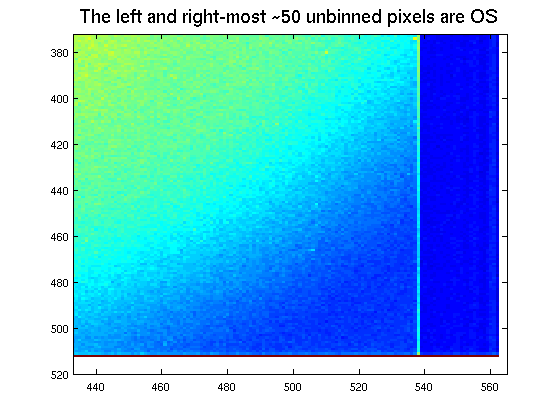
\includegraphics [width=4in]{ADA_1_loadnpreproc_p_03.png}


\subsection*{Bad-border}

\begin{par}
The top and bottom lines are way off-set
\end{par} \vspace{1em}
\begin{verbatim}
plot(d(1:4,:)')
\end{verbatim}

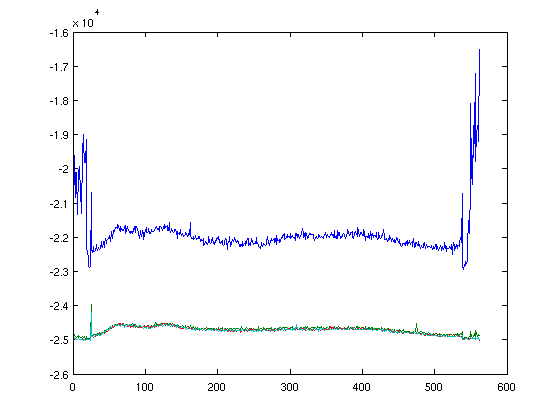
\includegraphics [width=4in]{ADA_1_loadnpreproc_p_04.png}


\subsection*{"Bad-pixels"}

\begin{par}
As in all CCDs there are a few bad pixels. That is they are either black, white, cold or hot.
\end{par} \vspace{1em}
\begin{verbatim}
imagesc(d)
caxis([-24566 -23866])
axis([149 397 226 421])
\end{verbatim}

\includegraphics [width=4in]{ADA_1_loadnpreproc_p_05.png}


\subsection*{Pre-processing}

\begin{par}
The normal way of reading ALIS data is to automatically do the necessary pre-processing steps, and possibly additional filtering. First get a default options struct
\end{par} \vspace{1em}
\begin{verbatim}
PO = typical_pre_proc_ops
% And change or set the parameters to accomodate the needs and whishes.
\end{verbatim}

\color{lightgray} \begin{verbatim}PO = 
                quadfix: 2
            quadfixsize: 0
          replaceborder: 1
              badpixfix: 1
             outimgsize: 0
           medianfilter: 3
            defaultccd6: 1
        bias_correction: 1
                  imreg: []
                  C_cam: []
     remove_these_stars: []
                 optpar: []
             size_r_t_s: 2
       v_interf_notches: []
                    psf: []
                    ffc: []
          fix_missalign: 1
                   verb: 0
     interference_level: Inf
    interference_method: 'flat'
       interference_swf: 3
             img_histeq: 0
              hist_crop: 0
            find_optpar: 1
\end{verbatim} \color{black}


\subsection*{Quadrant balancing}

\begin{verbatim}
d = quadfix3(d,2,abs(diff(size(d)))/2);
d = removerscanstrip(d,2,abs(diff(size(d)))/2);

imagesc(d),caxis([-25066 -23866]+25066)
title('Image after quadrant balancing','fontsize',16)
\end{verbatim}

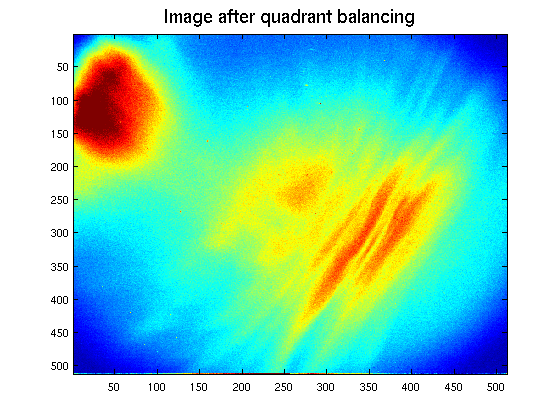
\includegraphics [width=4in]{ADA_1_loadnpreproc_p_06.png}


\subsection*{Adjusting the image borders}

\begin{verbatim}
d = replace_border(d);

imagesc(d),caxis([-25066 -23866]+25066)
title('and after correcting the border lines','fontsize',16)
\end{verbatim}

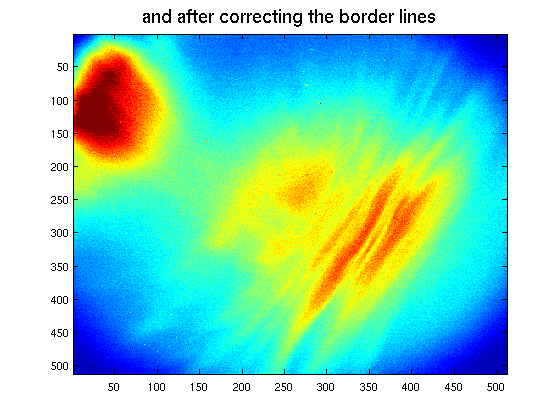
\includegraphics [width=4in]{ADA_1_loadnpreproc_p_07.png}


\subsection*{Correcting bad pixels}

\begin{par}
There is almost always good to correct the bad pixels
\end{par} \vspace{1em}
\begin{verbatim}
load cam1_badpix.dat
bp_tbl = cam1_badpix;
bpm = sparse(ceil(bp_tbl(:,2)/(1024/size(d,1))), ...
             ceil(bp_tbl(:,1)/(1024/size(d,2))), ...
             ones(size(bp_tbl(:,1))), ...
             size(d,1),size(d,2));
bpm = spones(bpm);
d = bad_pixel_fix(d,bpm);

imagesc(d),caxis([-25066 -23866]+25066)
title('and after correcting the bad pixels','fontsize',16)
\end{verbatim}

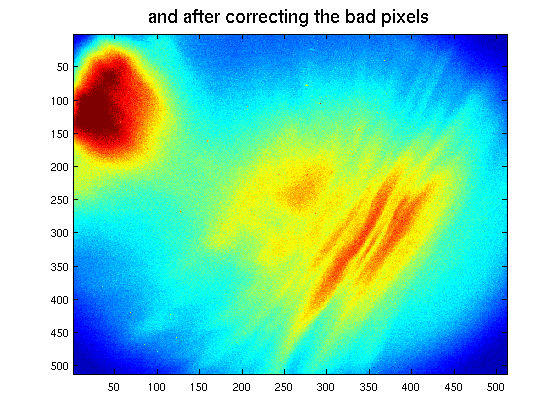
\includegraphics [width=4in]{ADA_1_loadnpreproc_p_08.png}


\subsection*{All in one go.}

\begin{verbatim}
[d,h,o] = inimg(filename,PO);

imagesc(d),caxis([-25066 -23866]+25066)
title('After typical preprocessing','fontsize',16)
\end{verbatim}

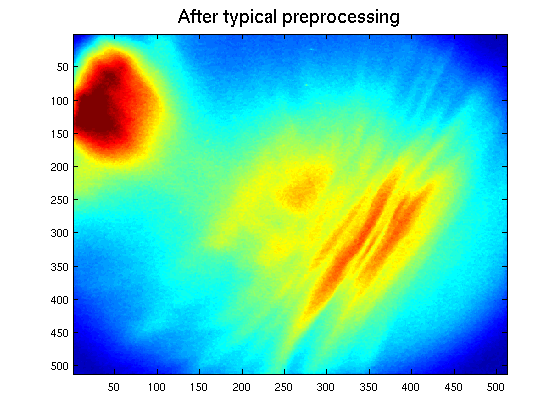
\includegraphics [width=4in]{ADA_1_loadnpreproc_p_09.png}



\end{document}
    
